\documentclass{beamer}

\title{Predstavitev naloge}

\date{\today}

\begin{document}

\setbeamertemplate{footline}[page number]
% 1. prosojnica: Uvodna prosojnica
\begin{frame}
  \titlepage
\end{frame}

% 2. prosojnica: Kazalo vsebine
\begin{frame}
  \frametitle{Kazalo vsebine}
  \begin{itemize}
    \item Predstavitev datoteke naloga1\_1.txt
    \item Graf P(t)
    \item Trapezna metoda za izračun integrala
  \end{itemize}
\end{frame}

% 3. prosojnica: Predstavitev datoteke naloga1_1.txt
\begin{frame}
  \frametitle{Predstavitev datoteke naloga1\_1.txt}
  \begin{itemize}
    \item V prvi vrstici datoteke je bil zapis: \\ time [s]
    \item V drugi vrstici je pisalo: stevilo preostalih  vrstic: \\
    100; stevilo podatkov v vrstici: 1
    \item Potem pa je bil niz števil od 0 do 1 z enakomernim razmikom med njimi
    \item Uporabil sem funkcijo: readtable, ki prebere podatke in jih shrani v tabelo.
    \item Vhodni podatki so čas v sekundah, izhod pa je vektor t, ki vsebuje te vrednosti.
  \end{itemize}
\end{frame}

% 4. prosojnica: Predstavitev grafa P(t)
\begin{frame}
  \frametitle{Graf P(t)}
  \begin{itemize}
    \item Predstavljen je graf, ki prikazuje odvisnost moči P od časa t.
  \end{itemize}
  \begin{figure}
    \centering
    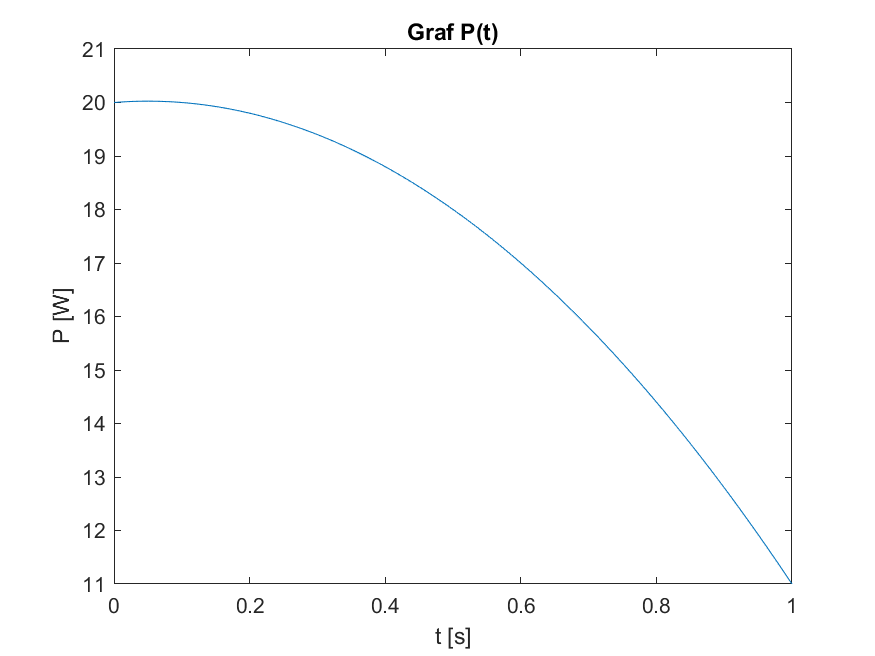
\includegraphics[width=0.8\textwidth]{graf.png} 
  \end{figure}
\end{frame}

% 5. prosojnica: Trapezna formula za integral
\begin{frame}
  \frametitle{Trapezna formula za integral}
  \begin{itemize}
    \item Trapezna formula za izračun integrala:
    \[
    \int_a^b f(x) \, dx = \frac{\Delta x}{2} \left( f(x_0) + 2 \sum_{i=1}^{n-1} f(x_i) + f(x_n) \right)
    \]
    \item MATLAB rešitev integrala s trapezno metodo:
    \[
     \text{int} =\sum_{i=2}^{n} \frac{(P(i) + P(i-1)) \cdot \Delta t}{2}
    \]
    \item Rezultat izračuna integrala je enak matlab funkciji trpz in je 17.1665Ws ali 4,49 mWh   
  \end{itemize}
\end{frame}

\end{document}

